% Options for packages loaded elsewhere
% Options for packages loaded elsewhere
\PassOptionsToPackage{unicode}{hyperref}
\PassOptionsToPackage{hyphens}{url}
\PassOptionsToPackage{dvipsnames,svgnames,x11names}{xcolor}
%
\documentclass[
]{article}
\usepackage{xcolor}
\usepackage[left=1in,right=1in,top=1in,bottom=1in]{geometry}
\usepackage{amsmath,amssymb}
\setcounter{secnumdepth}{-\maxdimen} % remove section numbering
\usepackage{iftex}
\ifPDFTeX
  \usepackage[T1]{fontenc}
  \usepackage[utf8]{inputenc}
  \usepackage{textcomp} % provide euro and other symbols
\else % if luatex or xetex
  \usepackage{unicode-math} % this also loads fontspec
  \defaultfontfeatures{Scale=MatchLowercase}
  \defaultfontfeatures[\rmfamily]{Ligatures=TeX,Scale=1}
\fi
\usepackage{lmodern}
\ifPDFTeX\else
  % xetex/luatex font selection
  \setmainfont[]{Latin Modern Roman}
\fi
% Use upquote if available, for straight quotes in verbatim environments
\IfFileExists{upquote.sty}{\usepackage{upquote}}{}
\IfFileExists{microtype.sty}{% use microtype if available
  \usepackage[]{microtype}
  \UseMicrotypeSet[protrusion]{basicmath} % disable protrusion for tt fonts
}{}
\makeatletter
\@ifundefined{KOMAClassName}{% if non-KOMA class
  \IfFileExists{parskip.sty}{%
    \usepackage{parskip}
  }{% else
    \setlength{\parindent}{0pt}
    \setlength{\parskip}{6pt plus 2pt minus 1pt}}
}{% if KOMA class
  \KOMAoptions{parskip=half}}
\makeatother
% Make \paragraph and \subparagraph free-standing
\makeatletter
\ifx\paragraph\undefined\else
  \let\oldparagraph\paragraph
  \renewcommand{\paragraph}{
    \@ifstar
      \xxxParagraphStar
      \xxxParagraphNoStar
  }
  \newcommand{\xxxParagraphStar}[1]{\oldparagraph*{#1}\mbox{}}
  \newcommand{\xxxParagraphNoStar}[1]{\oldparagraph{#1}\mbox{}}
\fi
\ifx\subparagraph\undefined\else
  \let\oldsubparagraph\subparagraph
  \renewcommand{\subparagraph}{
    \@ifstar
      \xxxSubParagraphStar
      \xxxSubParagraphNoStar
  }
  \newcommand{\xxxSubParagraphStar}[1]{\oldsubparagraph*{#1}\mbox{}}
  \newcommand{\xxxSubParagraphNoStar}[1]{\oldsubparagraph{#1}\mbox{}}
\fi
\makeatother


\usepackage{longtable,booktabs,array}
\usepackage{calc} % for calculating minipage widths
% Correct order of tables after \paragraph or \subparagraph
\usepackage{etoolbox}
\makeatletter
\patchcmd\longtable{\par}{\if@noskipsec\mbox{}\fi\par}{}{}
\makeatother
% Allow footnotes in longtable head/foot
\IfFileExists{footnotehyper.sty}{\usepackage{footnotehyper}}{\usepackage{footnote}}
\makesavenoteenv{longtable}
\usepackage{graphicx}
\makeatletter
\newsavebox\pandoc@box
\newcommand*\pandocbounded[1]{% scales image to fit in text height/width
  \sbox\pandoc@box{#1}%
  \Gscale@div\@tempa{\textheight}{\dimexpr\ht\pandoc@box+\dp\pandoc@box\relax}%
  \Gscale@div\@tempb{\linewidth}{\wd\pandoc@box}%
  \ifdim\@tempb\p@<\@tempa\p@\let\@tempa\@tempb\fi% select the smaller of both
  \ifdim\@tempa\p@<\p@\scalebox{\@tempa}{\usebox\pandoc@box}%
  \else\usebox{\pandoc@box}%
  \fi%
}
% Set default figure placement to htbp
\def\fps@figure{htbp}
\makeatother


% definitions for citeproc citations
\NewDocumentCommand\citeproctext{}{}
\NewDocumentCommand\citeproc{mm}{%
  \begingroup\def\citeproctext{#2}\cite{#1}\endgroup}
\makeatletter
 % allow citations to break across lines
 \let\@cite@ofmt\@firstofone
 % avoid brackets around text for \cite:
 \def\@biblabel#1{}
 \def\@cite#1#2{{#1\if@tempswa , #2\fi}}
\makeatother
\newlength{\cslhangindent}
\setlength{\cslhangindent}{1.5em}
\newlength{\csllabelwidth}
\setlength{\csllabelwidth}{3em}
\newenvironment{CSLReferences}[2] % #1 hanging-indent, #2 entry-spacing
 {\begin{list}{}{%
  \setlength{\itemindent}{0pt}
  \setlength{\leftmargin}{0pt}
  \setlength{\parsep}{0pt}
  % turn on hanging indent if param 1 is 1
  \ifodd #1
   \setlength{\leftmargin}{\cslhangindent}
   \setlength{\itemindent}{-1\cslhangindent}
  \fi
  % set entry spacing
  \setlength{\itemsep}{#2\baselineskip}}}
 {\end{list}}
\usepackage{calc}
\newcommand{\CSLBlock}[1]{\hfill\break\parbox[t]{\linewidth}{\strut\ignorespaces#1\strut}}
\newcommand{\CSLLeftMargin}[1]{\parbox[t]{\csllabelwidth}{\strut#1\strut}}
\newcommand{\CSLRightInline}[1]{\parbox[t]{\linewidth - \csllabelwidth}{\strut#1\strut}}
\newcommand{\CSLIndent}[1]{\hspace{\cslhangindent}#1}



\setlength{\emergencystretch}{3em} % prevent overfull lines

\providecommand{\tightlist}{%
  \setlength{\itemsep}{0pt}\setlength{\parskip}{0pt}}



 


\setlength{\footskip}{65pt}
\usepackage[font=scriptsize]{caption}
\usepackage[noblocks]{authblk}
\renewcommand*{\Authsep}{, }
\renewcommand*{\Authand}{, }
\renewcommand*{\Authands}{, }
\renewcommand\Affilfont{\small}
\renewcommand{\thefootnote}{\alph{footnote}}
\usepackage{etoolbox}
\AtEndEnvironment{abstract}{\noindent\textbf{Keywords:} \KeywordList \par}
\makeatletter
\@ifpackageloaded{caption}{}{\usepackage{caption}}
\AtBeginDocument{%
\ifdefined\contentsname
  \renewcommand*\contentsname{Table of contents}
\else
  \newcommand\contentsname{Table of contents}
\fi
\ifdefined\listfigurename
  \renewcommand*\listfigurename{List of Figures}
\else
  \newcommand\listfigurename{List of Figures}
\fi
\ifdefined\listtablename
  \renewcommand*\listtablename{List of Tables}
\else
  \newcommand\listtablename{List of Tables}
\fi
\ifdefined\figurename
  \renewcommand*\figurename{Figure}
\else
  \newcommand\figurename{Figure}
\fi
\ifdefined\tablename
  \renewcommand*\tablename{Table}
\else
  \newcommand\tablename{Table}
\fi
}
\@ifpackageloaded{float}{}{\usepackage{float}}
\floatstyle{ruled}
\@ifundefined{c@chapter}{\newfloat{codelisting}{h}{lop}}{\newfloat{codelisting}{h}{lop}[chapter]}
\floatname{codelisting}{Listing}
\newcommand*\listoflistings{\listof{codelisting}{List of Listings}}
\makeatother
\makeatletter
\makeatother
\makeatletter
\@ifpackageloaded{caption}{}{\usepackage{caption}}
\@ifpackageloaded{subcaption}{}{\usepackage{subcaption}}
\makeatother
\usepackage{bookmark}
\IfFileExists{xurl.sty}{\usepackage{xurl}}{} % add URL line breaks if available
\urlstyle{same}
\hypersetup{
  pdftitle={A test of higher and lower fractional volumes of resistance training upon arm and thigh muscle area: A multi-site randomised trial},
  pdfauthor={James Steele; David Gschneidner; Luke Carlson; James Fisher},
  pdfkeywords={resistance training, volume, hypertrophy, trained
participants},
  colorlinks=true,
  linkcolor={blue},
  filecolor={Maroon},
  citecolor={Blue},
  urlcolor={Blue},
  pdfcreator={LaTeX via pandoc}}


\title{A test of higher and lower fractional volumes of resistance
training upon arm and thigh muscle area: A multi-site randomised
trial\thanks{Preprint, please cite as: Steele, J., Gschneidner, D.,
Carlson, L., and Fisher, J. (2026). A test of higher and lower
fractional volumes of resistance training upon arm and thigh muscle
area: A multi-site randomised trial. sportrxiv DOI:
\url{https://doi.org/10.51224/SportRxiv.810}. Address for
correspondence: james@steele-research.com}}


\author[1,2,3,4]{James Steele}
\author[5]{David Gschneidner}
\author[5]{Luke Carlson}
\author[4,6,7]{James Fisher}

\affil[1]{Steele Research Limited, Eastleigh, Hampshire, UK}
\affil[2]{MacroFactor, Stronger by Science Technologies LLC, Raleigh,
North Carolina, USA}
\affil[3]{School of Health and Biomedical Sciences, Royal Melbourne
Institute of Technology, Melbourne, VIC, Australia}
\affil[4]{Department of Sport and Health, Solent University,
Southampton, Hampshire UK}
\affil[5]{Discover Strength, Minneapolis, Minnesota, USA}
\affil[6]{The Exercise Coach, Tennessee, USA}
\affil[7]{Department of Rehabilitation \& Sport Sciences, Bournemouth
University, Bournemouth, Dorset, UK}

% Store the keywords (expanded by Pandoc here)
\def\KeywordList{resistance training, volume, hypertrophy, trained
participants}

\date{April 10, 2026}
\begin{document}
\maketitle
\begin{abstract}
Recent work has theorised the effects of resistance training volume to
be positive and monotonic, albeit with diminishing returns, with regards
to hypertrophy. Improvements in muscle size however are typically small,
even smaller in trained people due to the linear-logarithmic adaptation
to RT over time, and thus between intervention differences in effects
are likely to be very small. As such, in contrast to most studies in the
field which aim to detect differences between interventions, we sought
to conduct a highly powered pre-registered test of the statistical
equivalence of two RT interventions in previously trained participants;
namely low (9 fractional sets per week) and high (36 fractional sets per
week) volumes. A randomised controlled trial across 22 sites was
employed with 125 partcipants recruited. Our primary outcome was
hypertrophy operationalised as estimated muscle cross sectional area
using circumference and skinfold measurements of the upper arm and
thigh. At the participant level, 120 participants were randomly assigned
to either the low (n = 56) or high (n = 64) volume RT intervention
condition. Participants underwent pre-intervention testing and then
participated in a 12-week intervention with post-intervention testing
following this. Our primary estimand of interest was the condition by
time interaction effect from our pre-registered analysis of pooled
outcomes reflecting the standardised between condition difference in
change in hypertrophy over time. After randomisation 112 participants
completed baseline testing and 87 completed post-intervention testing;
all data was used for analysis. The estimate for this effect was 0.023
{[}90\%CI: -0.044, 0.091{]} and the \emph{p}-value for equivalence was
\emph{p}=0.032 supporting statistically equivalent effects between
conditions. Main effects for time were also small 0.087 {[}95\%CI:
0.047, 0.128{]} in line with prior predictions from theoretical
linear-log growth models. This study is to our knowledge one of the
largest to compare the effects of low and high volume RT interventions
upon hypertrophy in previously trained participants. We found
statistical equivalence between both conditions and both main effects of
time, and any interaction effects for condition by time, are likely
small. More broadly, this study further corroborates the linear-log
theory of adaptation, that the effects of RT in trained persons should
be expected to be small, and that current studies in the field of RT are
woefully underpowered to be able to detect their effects, let alone test
between intervention comparisons.
\end{abstract}


\section{Introduction}\label{introduction}

A long-standing, though often debated, theory in resistance training
(RT) is that muscular hypertrophy is effected in some dose-response
fashion by the volume of RT performed. Indeed, the most recent
meta-regression analyses have estimated, with volume best
operationalised as fractional sets (i.e., whereby \emph{indirect}
exercises count for half of a set towards volume for that muscle group,
and \emph{direct} count as a whole set), a positive monotonic
dose-response relationship, albeit with diminishing returns, between
both weekly (Pelland et al., 2026), and per session (Remmert et al.,
2025), set volumes and muscle hypertrophy. From a practical perspective,
these meta-regressions suggest \textasciitilde11 fractional sets per
session with \textasciitilde31 weekly fractional sets before there is no
additionally detectable superiority to greater volumes. This corresponds
to a recommendation of \textasciitilde3 sessions per week performing
\textasciitilde11 sets per session. In terms of the estimated
magnitudes, for example, the standardised mean difference (SMD) for a
contrast of 9 fractional sets per week against 36 fractional sets per
week\footnote{Note these are provided as the example as these are the
  volumes examined in the present study.} is 0.294 {[}95\% CI: 0.20,
0.39{]}. Further, the dose-response effect estimated by these
meta-regressions does not appear to be moderated by training status
which suggests that we should predict, based on this theory, that there
are still benefits for higher volumes in trained participants and of a
similar comparative magnitude. However, though larger than typical, the
meta-regressions supporting this theory of dose-response to RT volume
included only k=35 studies on hypertrophy outcomes and the lack of
conditional effects by training status combined with contrasts of this
magnitude seem unrealistic in light of other background knowledge and
theory.

When we contextualise this contrast effect of fractional volume with the
findings of a larger meta-analysis (k=111) of varied RT interventions
compared to non-training controls in untrained participants, which has
estimated the typical effect of RT upon hypertrophy to be only 0.34
{[}95\% confidence interval: 0.29, 0.39{]} SMD (Steele et al., 2023),
the estimated effects for higher volumes seem comparatively large.
Further, previous work has demonstrated that RT outcomes respond in a
roughly linear-log function with duration of exposure to RT suggesting
diminished effects with greater prior training exposure (Latella et al.,
2024; Steele et al., 2022) \footnote{See also the results of an
  arm-based meta-regression model examining the time-course of
  adaptation in the data from the aforementioned large meta-analysis
  (Steele et al., 2023) (see \url{https://osf.io/7fdvq})}. Given this,
it seems likely that the simple training effect for any RT intervention
over time in previously trained participants for the typical duration
(i.e., \textasciitilde12 weeks) of a study is far less than the 0.34 SMD
noted above. In fact, given this theory of linear-log adaptation, the
estimated contrast when using the large meta-analysis data set mentioned
(Steele et al., 2023) reveals a simple training effect prediction over
time of \textasciitilde{} 0.05 SMD for participants with at least 6
months of prior training engaging in a further 12 week intervention
duration. Corroborating this theory of linear-log adaptation, and the
magnitudes of effects it predicts, the estimates for both the main
effect of time, and time-by-condition interaction, were very close to
the \emph{a priori} predictions based on this theories derivation chain
in a recent large sample pre-registered study of ours in trained
participants (Gschneidner et al., 2025).

Whilst the theory that there may be a positive monotonic dose-response
effect of fractional volumes upon muscle hypertrophy may in fact be
true, it seems unlikely that any between-volume differences are of the
magnitudes suggested in recent meta-regressions when examining
previously trained participants. Researchers designing studies to act as
strong tests of the theory of positive monotonic dose-response effects
with RT volume in trained persons should also pay heed to the well
corroborated theory of linear-log adaptation with duration of exposure
to RT. As such, they should expect the magnitude of effects when
comparing volumes to be small, even if real, in trained participants.
Indeed, given the predicted main effects of time for RT, it seems
unlikely that any difference between two RT interventions of different
fractional volumes would even reach any reasonable smallest effect size
of interest (SESOI). In our recent work we have begun to anticipate this
and, following recent arguments for this in the sport and exercise
sciences (Mazzolari et al., 2022), plan to test for equivalence within a
defined SESOI (an SMD of {[}-0.1, 0.1{]}) instead of testing for the
presence of an effect against a point null hypothesis of no difference
(Gschneidner et al., 2025).

Thus, whilst RT volume may indeed have a true effect upon muscle
hypertrophy, this effect must necessarily be very small. As such, we
sought to conduct a pre-registered test of the equivalence of two RT
interventions of differing fractional weekly set volumes in previously
trained participants. Our hypothesis was thus; in participants with at
least 6 months of prior resistance training experience completing a 12
week intervention, the higher fractional volume resistance training
condition will produce changes over time in our primary outcome measure
of estimated muscle size (measured for both arm and thigh standardised
and pooled across studies; see statistical analysis below) that are not
larger (or smaller) than the SESOI when compared with the lower
fractional volume resistance training intervention condition i.e., will
be statistically equivalent.

\section{Methods}\label{methods}

\subsection{Experimental approach to the
problem}\label{experimental-approach-to-the-problem}

A randomised controlled trial across multiple sites was employed. At the
participant level, participants were randomly assigned to either the low
volume or high volume RT intervention condition. Participants underwent
baseline testing (t\textsubscript{0}) and then participated in a 12-week
intervention with post testing following the 12-week intervention
(t\textsubscript{1}). This study was pre-registered June 2025, available
at: \url{https://doi.org/10.17605/OSF.IO/7VMXK}. This study was covered
under prior ethical approval by Solent University Health, Exercise, and
Sports Science Research Ethics and Innovation Committee (reference
number: fishj1HESS2024).

\subsection{Updates to
pre-registration}\label{updates-to-pre-registration}

Note, our pre-registration underwent several updates which are
documented clearly in the pre-registration due to both logistical
reasons and some errors noticed in the original simulations and sample
size planning. To summarise here for the reader, three major updates are
relevant to highlight. Firstly, due to a clerical error some
participants in the low volume group began the intervention period
undertaking an earlier version of the proposed low volume intervention
and as such it was decided to halt the study, allow a one-week washout
of no training/testing, and then have them restart including baseline
testing again. Secondly, due to an error in the original simulations for
determination of sample size we realised that our original target for
sample size would be insufficient to achieve acceptable power given the
originally chosen and very conservative type 1 error rate
(\(\alpha=0.01\)). As such, after changing our analysis plan to the most
powerful option from our simulations we also opted to increase our type
1 error rate to the more traditional rate utilised in the field
(\(\alpha=0.05\)) in order to enable us to achieve sufficient
statistical power (i.e., \textasciitilde80\%). Lastly, as in our
previous study (Gschneidner et al., 2025) we originally planned to
utilise structured client workout records using StrengthPortal; however,
prior to the study launch Discover Strength stopped using this software.
As such, workout records were manually recorded across sites via
googlesheet workout cards. This resulted in a large amount of
unstructured workout data and, as this would have required a
considerable amount of manual work to restructure, clean, and prepare
this data, the decision was made to omit the secondary outcomes for
strength as estimated 1RM from our analysis. Note, the methods described
here pertain to the updated pre-registered methods.

\subsection{Participants and Sample
Size}\label{participants-and-sample-size}

Our pre-registered target sample size for recruitment was 120
participants (across 24 Discover Strength sites, target of 5
participants recruited at each site). The full details of the updated
sample size justification for statistical power including simulations,
assumptions, analyses, and inference criteria can be seen in the
pre-registration. Briefly, we assumed the aforementioned theoretical
linear-log growth function and estimated the expected main effect of
time (SMD of \textasciitilde0.05) for participants with the prior
training experience required for inclusion, noted below, and assumed any
condition by time interaction effect to be at most half of this (i.e.,
\textasciitilde0.025). We considered this to be within what we felt to
be the SESOI for changes in estimated muscle size; an SMD ranging
{[}-0.1, 0.1{]}. We also corroborated the choice of this SESOI by
consulting other researchers in the area and have utilised this in
previous work (Gschneidner et al., 2025; Varovic et al., 2025). We then
simulated to determine statistical power at different sample sizes
assuming these effects, assuming a dropout rate of \textasciitilde15\%
based on our previous studies (Carlson et al., 2023; Gschneidner et al.,
2025), and testing for equivalence following the analysis plan detailed
below.

A total of 125 participants (mean±sd: age = 33±14 years, body mass =
81.96±14.78 kilograms, height = 176.62±9.96 centimetres; and 41 females
and 84 males) were recruited from 22 locations of Discover Strength
personal training studio (USA). A total of 120 participants were
randomised to either the low (n = 56) or high volume conditions (n =
64). All participants were existing clients or staff with a minimum of 6
months RT experience with Discover Strength (though may have also had
prior training experience before joining Discover Strength as members;
self-reported total prior RT experience including at least 6 months of
experience at Discover Strength was 11±7 years (mean±sd) ensuring all
participants were of a similar recent training background prior to
participation. As such, all participants prior to beginning the study
had been training for at least 6 months with supervised, high effort
(i.e., training to momentary failure, and occasionally the use of the
use of advanced training techniques such as drop-sets, pre- or
post-exhaustion, forced repetitions, rest-pause etc.), low-volume (i.e.,
a single set of each exercise), and twice-weekly training sessions.
Participants were instructed not to (and confirmed with supervising
trainers that they did not), engage in any muscle strengthening exercise
outside of their supervised RT sessions. Participants were also asked to
maintain normal dietary patterns and daily activities or other physical
activities, exercise, and sports that they currently participated in
(e.g., not to begin additional exercise strategies to enhance weight
loss/gain). All participants signed an informed consent form prior to
any data collection.

\subsection{Muscle Area Measurement}\label{muscle-area-measurement}

The primary outcome was muscle hypertrophy operationalised as arm- and
thigh- muscle area estimated from anthropometric measurements with at
least 72 hours between post testing and the final training session.
Estimates of both arm muscle cross sectional area (CSA) and thigh muscle
CSA were made from anthropometric measurements using methods and
equations described previously by Heymsfield, et al. (1982) and Housh et
al. (1995), respectively. For arm muscle CSA, circumference was measured
at the midpoint between the tip of the acromion and the olecranon
process with the arm hanging relaxed by the participant's side and
taking the triceps skinfold as a vertical fold at the same point using
callipers. For thigh muscle CSA, circumference was measured at the
midpoint of the inguinal crease and the proximal border of the patella,
and a thigh skinfold taken as a vertical fold at the same point using
the same callipers. Measurements were taken by multiple instructors
across multiple locations. All staff at each site conducting
anthropometric measurements underwent initial training collecting
measurements from at least 5 different people over two occasions. For
each muscle CSA outcome three measurements were taken for both
circumference and skinfold at each time point and all were used in
analysis. This choice was based on simulations in planning our previous
study (Gschneidner et al., 2025) regarding the impact of multiple
measurements at each time point, whilst taking into account estimated
measurement error determined from prior data, upon statistical power.
Baseline test-retest data from our previous study (Gschneidner et al.,
2025) estimated the standard error of measurement for estimated arm and
thigh CSA to be 4.62 \(\textrm{cm}^2\) and 7.97 \(\textrm{cm}^2\)
respectively.

Similarly to our previous study, our choice for these methods of
operationalisation is pragmatic as, given the scale of the study being
conducted across multiple sites, in order to reach sufficient sample
size for statistical power we are limited in our ability to collect more
direct measures such as ultrasound by the availability of equipment and
trained personnel to collect that data. Indeed, Haun et al. (2019) have
argued that, while such measurements might not offer microscopic
insights into myofibrillar protein accrual or functional CSA, they are
appropriate for examining changes due to RT interventions and
particularly so when resource and technical constraints prevent the use
of other methods. Further, we had previously reported (Gschneidner et
al., 2025) a re-analysis of data for 67 participants (both untrained and
trained) from a previous collection of studies where both circumference
and ultrasound-based measures of hypertrophy had been used (Gentil et
al., 2020). Calculating the pre- to post-intervention SMDs for both
methods, and then comparing the methods using a random effects
meta-analysis with method as a moderator revealed an SMD for
circumference measures of 0.34 {[}95\%CI: 0.23, 0.44{]}, for ultrasound
measures of 0.27 {[}95\%CI: 0.19, 0.35{]}, and difference between
methods of -0.07 {[}95\%CI: -0.2, 0.06{]}. Thus, both methods appear
clearly able to detect changes in muscle size with relatively similar
effect size magnitudes suggesting that the estimated CSA method used in
this study are valid for their purpose.

\subsection{Intervention}\label{intervention}

For both training intervention conditions (i.e., low and high volume)
participants trained with a load permitting \textasciitilde7-10
repetitions to be completed before reaching momentary failure (defined
as the point at which, despite the greatest effort, the participant
failed to complete the concentric phase of a repetition (Steele et al.,
2017)) using a repetition duration of 2 second concentric and 4 second
eccentric actions. The high volume condition had load altered in
subsequent sets within the same session by the supervising trainer to
enable an approximately similar repetition range to be achieved for each
set. Both conditions performed three sessions a week for 12 weeks.
Unless specified the exercises were performed using resistance machines
(combination of MedX, Imagine Strength, Nautilus, and Hammer Strength
depending on the available equipment at the site).

The high volume condition, in each session, performed the following
workout of 12 fractional sets for the upper arm, and 12 fractional sets
for the thigh, totalling 36 fractional sets for both upper arm and thigh
per week:

\begin{itemize}
\tightlist
\item
  3 sets of Leg Press (direct sets)
\item
  3 sets of Leg Curl (direct sets)
\item
  3 sets of Leg Extension (direct sets)
\item
  3 sets of Barbell/Dumbbell Romanian Deadlift (direct sets)
\item
  2 sets of Chest Press (indirect sets)
\item
  2 sets of Pulldown (indirect sets)
\item
  2 sets of Dumbbell Skullcrusher (direct sets)
\item
  2 sets of Dumbbell Split Stance Biceps Curl (direct sets)
\item
  2 sets of Overhead Press (indirect sets)
\item
  2 sets of Seated Row (indirect sets)
\item
  2 sets of Dumbbell French Press Tricep Extension (direct sets)
\item
  2 sets of Dumbbell Hammer Incline Curl (direct sets)
\end{itemize}

The low volume condition, in each session, performed one of the two
following workouts in alternation consisting of 3 fractional sets for
the upper arm, and 3 fractional sets for the thigh, totalling 9
fractional sets for both upper arm and thigh per week utilising the same
core direct and indirect sets exercise selection as the high volume
condition (in addition they completed a selection of exercises not
directly or indirectly targeting the upper arm or thigh in order to
increase the total session duration to be similar to typical session
durations and accommodate the logistics of session timetabling at
Discover Strength):

Workout A

\begin{itemize}
\tightlist
\item
  1 set of Leg Press (direct set)
\item
  1 set of Leg Curl (direct set)
\item
  1 set of Leg Extension (direct set)
\item
  1 set of Tibia Dorsiflexion
\item
  1 set of Pec Fly
\item
  1 set of Pullover
\item
  1 set of Chest Press (indirect set)
\item
  1 set of Pulldown (indirect set)
\item
  1 set of Dumbbell French Press Tricep Extension (direct set)
\item
  1 set of Dumbbell Split Stance Biceps Curl (direct set)
\item
  1 set of Abdominal Flexion
\item
  1 set of Lumbar Extension
\end{itemize}

Workout B

\begin{itemize}
\tightlist
\item
  1 set of Seated Calf Raise i.e., Plantarflexion
\item
  1 set of Leg Press (direct set)
\item
  1 set of Barbell/Dumbbell Romanian Deadlift (direct set)
\item
  1 set of Leg Extension (direct set)
\item
  1 set of Overhead Press (indirect set)
\item
  1 set of Seated Row (indirect set)
\item
  1 set of Shoulder Lateral Raise
\item
  1 set of Rear Shoulder Raise
\item
  1 set of Dumbbell French Press Tricep Extension (direct set)
\item
  1 set of Dumbbell Split Stance Biceps Curl (direct set)
\item
  1 set of Torso Rotation
\end{itemize}

The exercises selected were deemed to be either direct or indirect sets
regarding fractional volumes based upon the coding systems employed by
Pelland et al. (2026) and Remmert et al. (2025) in their
meta-regressions. Notably, our outcome measures pertained to the mid
point of the upper arm and thigh as a whole, and so we considered this
to include both elbow flexors/extensors, and knee flexors/extensors.
Hence, we have considered exercises that are direct/indirect for either
quadriceps, knee extensors, lateral thigh, anterior/middle thigh, vastus
lateralis, vastus medialis, vastus intermedius, hamstrings or posterior
thigh to be direct/indirect for the thigh as a whole, and exercises that
are direct/indirect for either triceps brachii, elbow extensors, biceps
brachii or elbow flexors to be direct/indirect for the upper arm as a
whole. We corresponded with these authors to confirm that our approach
reflected their coding sufficiently for our test of their volume model
to be valid.

\subsection{Statistical Analysis}\label{statistical-analysis}

All code utilized for data preparation and analyses are available in
either the Open Science Framework page for this project
\url{https://osf.io/bxa8p} or the corresponding GitHub repository
\url{https://github.com/jamessteeleii/project_DS_volume}. We cite all
software and packages used in the analysis pipeline using the
\texttt{grateful} package (Rodriguez-Sanchez et al., 2023) which can be
seen here:
\url{https://jamessteeleii.github.io/project_DS_volume/grateful-report.html}.

As noted, the project was previously pre-registered including the
analysis plan, model to be employed, parameter of primary interest, and
specific hypothesis relating to this. The full details of this including
the derivation of our hypotheses from prior evidence and theory
regarding the expected effects of resistance training upon hypertrophy
are fully detailed in the pre-registration for the reader (see
\url{https://doi.org/10.17605/OSF.IO/7VMXK}). Here we reiterate our
primary hypothesis related to the between condition comparison of low
vs.~high volume RT interventions upon muscle hypertrophy operationalised
as arm and thigh estimated muscle CSA over time i.e., the
time-by-condition interaction, where time is pre- and post-intervention
(i.e., t\textsubscript{0} and t\textsubscript{1}) and condition is the
two aforementioned interventions. We tested for the equivalence of the
slopes for time of high volume against the low volume comparator with a
SESOI of 0.1 SMD. Our hypothesis is thus that the high volume resistance
training condition will produce changes over time in our primary outcome
of muscle hypertrophy that are not larger (or smaller) than the SESOI
when compared with the low volume resistance training intervention
condition. More specifically:

\textbf{H0}: The interaction effect for time (pre- and
post-intervention) and condition (high fractional volume i.e., 36
fractional sets per week, or low fractional volume i.e., 9 fractional
sets per week) for standardised (i.e., z-scored) estimated muscle area
will differ from the smallest effect size of interest - upper and lower
bound of confidence interval for between condition effect will be
outside of or include the upper or lower limits of smallest effect size
of interest i.e., {[}-0.1,0.1{]}.

\textbf{H1}:The interaction effect for time (pre- and post-intervention)
and condition (high fractional volume i.e., 36 fractional sets per week,
or low fractional volume i.e., 9 fractional sets per week) for
standardised (i.e., z-scored) estimated muscle area will be equivalent
to the smallest effect size of interest - upper and lower bound of
confidence interval for between condition effect will be inside the
upper or lower limits of smallest effect size of interest i.e.,
{[}-0.1,0.1{]}.

An analysis of covariance as a linear mixed effects location-scale model
was fit using the \texttt{glmmTMB} package and using Restricted Maximum
Likelihood estimation for pooled standardised arm and thigh estimated
muscle CSA outcomes. We included fixed effects for time and
condition:time interaction (our estimate of interest), random intercepts
for both site id and participant id, for the location component (i.e.,
\(\mu_i\)). The scale component (i.e., \(\sigma_{i}^2\)) of the model
was to allow for heterogeneous variances between the two outcome
measures, as they were modelled as pooled, and so included a fixed
effect for outcome i.e., arm or thigh estimated muscle CSA. The model
equation was as follows:

\[
\begin{aligned}
\textrm{y}_{i} &\sim \mathcal{N}(\mu_i, \sigma_i^2) \\
\mu_i &= \beta_0
   + \beta_1 \, (\textrm{time}_i)
   + \beta_2 \, (\textrm{time}_i \times \textrm{condition}_i)
   + u_{j_[i]} + v_{k[i]} \\
u_j &\sim N(0, \sigma^2_{\text{participant}})
\quad \text{for participant } j = 1, \dots, J \\
v_k &\sim N(0, \sigma^2_{\text{site}})
\quad \text{for site } k = 1, \dots, K \\
\log(\sigma_i^2) &= \delta_0 + \delta_1 \, (\textrm{outcome}_i)
\end{aligned}
\]

Where \(\textrm{y}_{i}\) was the estimated muscle CSA for either arm or
thigh standardised following the approach of Penney (2023) i.e., using
the error term of a simple linear model including only the randomised
condition predictor avoiding possible attenuation issues with using
z-scores\footnote{Note, we deviate slightly from our pre-registered
  analysis here in that, instead of using the sample data to generate
  the denominator for standardising the estimated muscle CSA for either
  arm or thigh for analysis, we utilised the same denominators as
  estimated in our previous study (Gschneidner et al., 2025). The
  reasoning for this was that, given the nature of the present study, we
  had a comparatively smaller sample and so reasoned that the estimated
  \(\sigma\) from our previous and larger sample study was a better
  estimate. It would also render our results comparable with our
  previous study in terms of their exact magnitude. Notably, we realised
  in hindsight that we should have pre-registered this given that we
  anticipated more difficulty in recruitment and that we would not be
  able to obtain a sample size of the scale in our previous study given
  the nature of the interventions being examined in this population.}.
Condition was coded as centred (i.e., low = -0.5; high = 0.5) such that
the main effect of time was interpretable as the mean effect across both
conditions.

Our primary test for equivalence was upon the condition:time effect
i.e.,
\(\beta_{2}(\operatorname{time}_i \times \operatorname{condition}_i)\)
from our primary pre-registered model using the \texttt{marginaleffects}
packages \texttt{hypotheses()} function against our SESOI of 0.1. As
noted, we originally pre-registered \(\alpha=0.01\) to draw inferences
regarding equivalence, but this was updated to \(\alpha=0.05\) in order
to maximise statistical power for our test. We also examined the
estimated main time effect i.e., \(\beta_{1}(\operatorname{time})\) in
our model descriptively in terms of it's magnitude and precision, and
for visualisation present the un-pooled linear predictions for each
participant on the raw scale (i.e., cm\(^2\)) in addition to the means
and 95\% quantile intervals for the raw pre- and post-intervention data.

\section{Results}\label{results}

After randomisation a total of 112 participants underwent baseline
testing (lower volume = 53; higher volume = 59) and 87 (lower volume =
42; higher volume = 45) participants completed post-testing. There was
little difference in drop-out between conditions (low minus high volume
= -5\% {[}95\%CI: -21\%, 11\%{]}; low volume drop-out = 25\% {[}95\%CI:
13\%, 37\%{]}; high volume drop-out = 30\% {[}95\%CI: 19\%, 41\%{]}.

Our primary estimand of interest was the condition:time interaction
effect from our pre-registered analysis reflecting the between condition
difference in change in hypertrophy over time. The estimate for this
effect was a standardised value of 0.023 {[}90\%CI: -0.045, 0.091{]}.
The \emph{p}-value for equivalence was \emph{p}=0.032. As such,
considering our updated inference criteria with alpha set at 0.05, we
were able to reject the null hypothesis that the condition:time
interaction effect was outside of the SESOI {[}-0.1, 0.1{]} and thus
claim statistical equivalence of effects. The raw estimated muscle CSA
pre- and post-intervention predictions from un-pooled participant level
linear regression in addition to the means and 95\% quantile intervals
can be see in Figure~\ref{fig-hypertrophy-plot}, along with the
estimates for the main effect of time and condition:time interaction
effect on the standardised scale from the pre-registered model.

\begin{figure}

\centering{

\pandocbounded{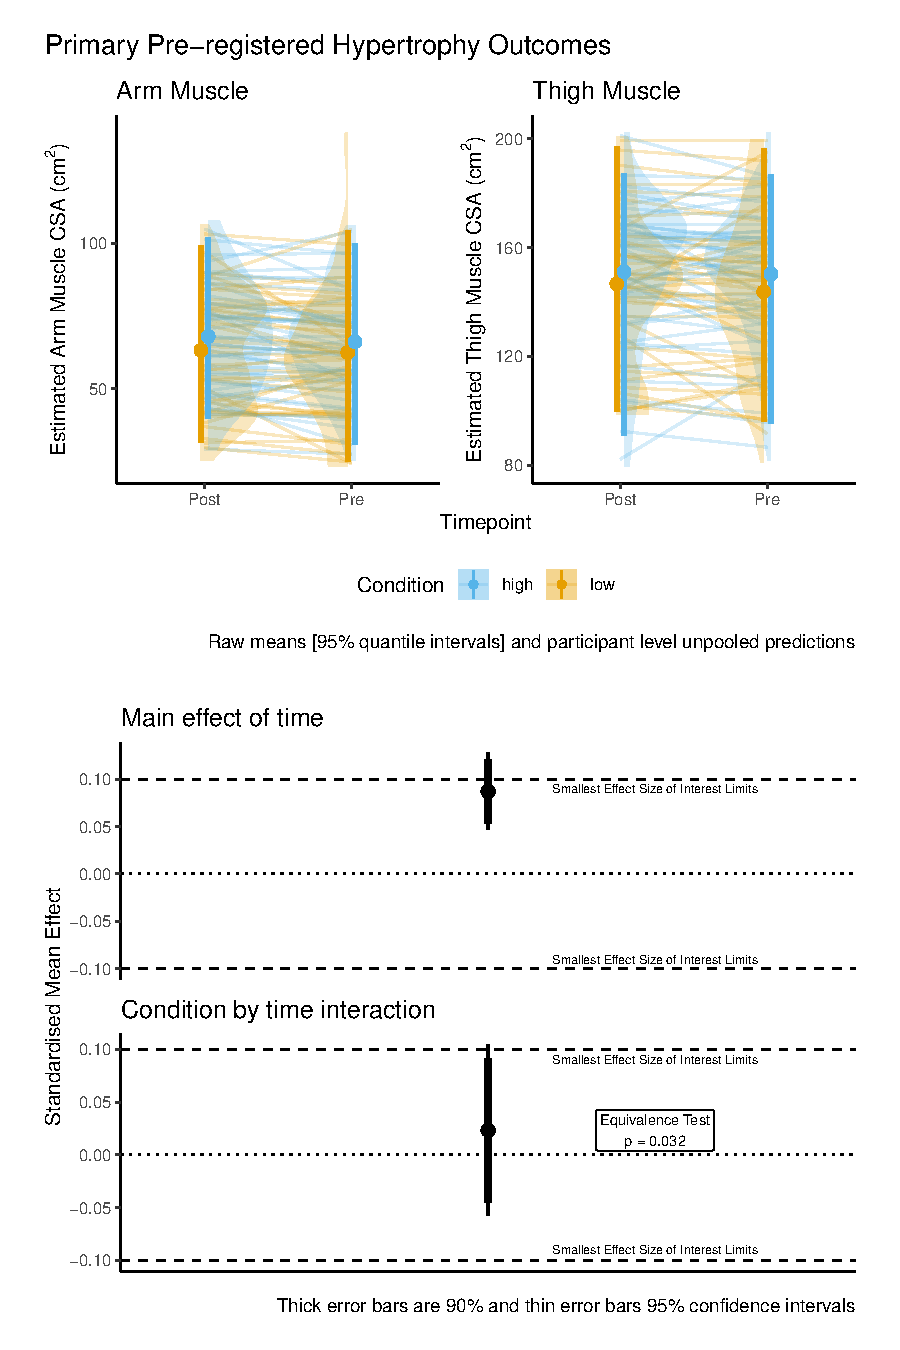
\includegraphics[keepaspectratio]{pre_print_files/figure-pdf/fig-hypertrophy-plot-1.pdf}}

}

\caption{\label{fig-hypertrophy-plot}Primary pre-registered hypertrophy
outcomes. The top two panels show raw estimated muscle CSA pre- and
post-intervention predictions from un-pooled participant level linear
regression in addition to means and 95\% quantile intervals. The bottom
two panels show estimates with 90\% and 95\% confidence intervals on the
standardised scale from the pre-registered model for the main effect of
time and condition:time interaction effect. The grey band on the main
effect of time plot shows the 95\% confidence interval for the effect
predicted from the linear-log meta-regression of hypertrophy outcomes in
previous studies estimated from (Steele et al., 2023), and the grey line
on the condition:time interaction plot shows the predicted between
condition contrast.}

\end{figure}%

\section{Discussion}\label{discussion}

To our knowledge this is the largest study to have experimentally
compared different RT volumes and offer a severe test (i.e., well
powered, pre-registered) of the combined theories regarding the
dose-response effects of RT volume and the linear-log adaptation to RT
over time for hypertrophy. In a multi-site randomized trial we compared
the effects of RT using low or high fractional weekly volumes upon
muscle size in trained participants and tested for equivalence. The
\emph{p}-value for equivalence was 0.032 supporting that the effects of
the low and high volume conditions examined were statistically
equivalent in trained participants (SMD = 0.023 {[}90\%CI: -0.045,
0.091{]}).

The overall magnitude of RT effect in trained participants seen in the
main effect of time in our models was 0.087 {[}95\%CI: 0.047, 0.128{]}
which was not dissimilar to the estimates reported in our previous work
(0.034 {[}95\%CI: 0.021, 0.046{]} and 0.051 {[}95\%CI: 0.037, 0.064{]}
for arm and thigh muscle respectively (Gschneidner et al., 2025). This,
combined with the statistical equivalence of the low and high volume
conditions, further corroborate the theory that adaptation is diminished
with continued participation in RT. Indeed, as this and our previous
work show, the main effects of RT are likely far smaller than the
typical studies in the field are designed to detect, let alone any
between condition comparative effects.

Although we report statistical equivalence within the range of our SESOI
in this study, it may remain a possibility that the theory of positive
monotonic dose response effects of RT volume do indeed continue to play
out in trained participants and perhaps it is just the case that the
effects are very small. It could be argued that true small effects
favouring higher volumes may yet still exist and that our study was
unable to detect them. It is assuredly the case that our study would
have been underpowered to detect very small effects and indeed alongside
our simulations to determine power at different sample sizes when
testing for equivalence we also examined power to test for the presence
of a very small between condition effect i.e., \textasciitilde0.025.
Such an effect would require \textgreater1000 participants to detect
with even modest statistical power of \textasciitilde60-70\% (see
\url{https://osf.io/z8vck}). As such, whilst we cannot rule out that for
a smaller SESOI we might not be able to infer statistical equivalence,
it remains incumbent for those researchers who might want to claim that
such small effects exist, and are important to detect, to conduct the
appropriate studies to provide a strong test of that claim or estimate
the effect with sufficient precision. From a practical perspective
trainees and trainers might opt to take our results at face value and
act as though both lower and higher volumes of the sort examined here
are indeed equivalent in effects and then opt to train one way or the
other based upon personal preference or other considerations.
Alternatively, if they believe that there may still be greater benefits
for higher volumes and do not see the additional time/resource
commitment or other costs associated with such RT to be sufficient to
dissuade them from engaging in it, then they may wish to pursue this
kind of training for the possibility that it \emph{may} provide them
with additional hypertrophy. However, strong claims to the effect that
higher volumes produce meaningfully greater hypertrophy than lower
volumes in trained participants are currently unwarranted in our
opinion.

The strengths of this study includes its sample size and
pre-registration. Yet, despite this, we will pre-empt (and indeed
reiterate given these have been highlighted already in our previous
work; (Gschneidner et al., 2025)) some of the limitations that might be
noted by readers. These include drop-outs and our chosen outcome
operationalisations.

We noted the update to our pre-registration and inference criteria in
order to maintain the desired statistical power. However, though in our
previous studies with Discover Strength members we estimated a dropout
rate of \textasciitilde15\% (Carlson et al., 2023; Gschneidner et al.,
2025) and accounted for this in our simulations, the rate observed in
the present study was almost double that. Fortunately there was not a
clear difference between the low and high volume groups in terms of
drop-outs and so we at least feel confident that differential drop-outs
have likely not biased our estimates substantially. The drop-outs will
have affected our statistical power and precision of our estimates,
though even in light of this the present study remains one of the
largest experimental trials of RT and the effects of volume. We
speculate that the higher drop-out rate in this study may have been due
to the increase in training frequency from the typical two sessions per
week that Discover Strength usually employ to three sessions per week
and the subsequent burden on participants.

Again, some may suggest that the operationalisations used for
hypertrophy (i.e., estimated muscle CSA from circumference and
skinfolds) in this study are not gold-standard and thus will have less
resolution to detect effects due to greater measurement error. However,
similarly to our previous work, we acknowledged this in study planning
and explicitly estimated the measurement error with our prior data using
these methods, used this in simulating to determine sample size for the
desired statistical power, and also made use of multiple measurements to
account for the error associated with single measurements. Additionally,
where in our previous work we modelled arm and thigh outcomes separately
and opted to adjust our alpha levels given our global hypothesis
regarding ``hypertrophy'' as an outcome, here we pooled standardised
outcomes and modelled these using an appropriate location-scale model
allowing for heterogeneous variances and providing greater statistical
power. Again, we feel confident that our operationalisations reflect the
construct of interest i.e., hypertrophy (Haun et al., 2019), given the
striking closeness of our estimates to the \emph{a priori} predictions
regarding the effects; predictions which were derived from both theory
and empirical evidence which had employed a wide range of
operationalisations for both constructs.

\section{Conclusion}\label{conclusion}

This study is, to our knowledge, one of the largest to compare the
effects of low and high volume RT interventions upon hypertrophy in
previously trained participants. We found statistical equivalence
between both conditions and both main effects of time, and any
interaction effects for condition by time, are likely small. More
broadly, this study further corroborates the linear-log theory of
adaptation, that the effects of RT in trained persons should be expected
to be small, and that current studies in the field of RT are woefully
underpowered to be able to detect their effects, let alone test between
intervention comparisons.

\section{Acknowledgements}\label{acknowledgements}

We would like to extend our sincere gratitude to all the Exercise
Physiologists at Discover Strength without whom this project would not
have been possible. Further, we would like to thank all participants in
this research study for their engagement in this project and their
commitment to their long-term health.

\section{Funding Information}\label{funding-information}

No direct funding was received for this study. Operational costs for its
delivery were absorbed by Discover Strength and so provided
\emph{in-kind} value.

\section{Author Contributions}\label{author-contributions}

JS, DG, LC, and JF conceived the idea for the project and designed the
methods. LC and DG coordinated and oversaw the data collection. JS
conducted the statistical analyses and produced data visualisations. JS
drafted the initial manuscript. JS, DG, LC, and JF contributed to
editing the manuscript. All authors read and approved the final
manuscript.

\section{Competing Interests}\label{competing-interests}

LC and DG work for Discover Strength. JF provides research consulting
for organizations within the health and fitness field and has received
travel expenses and honoraria for speaking and consulting with Discover
Strength. JS provides research consultancy through his company Steele
Research Limited, is contracted currently by MacroFactor and Kieser
Australia through Steele Research Limited, and has also received travel
expenses and honoraria for speaking from fit20 International, Exercise
School Portugal, and Discover Strength.

The content does not necessarily represent the official views of the
affiliations or contracting organisations listed.

\section{Data and Supplementary Material
Accessibility}\label{data-and-supplementary-material-accessibility}

All data and code utilised for data preparation and analyses are
available in either the Open Science Framework page for this project
\url{https://osf.io/bxa8p/overview} or the corresponding GitHub
repository \url{https://github.com/jamessteeleii/project_DS_volume}.

\section{References}\label{references}

\phantomsection\label{refs}
\begin{CSLReferences}{1}{0}
\bibitem[\citeproctext]{ref-carlsonEffectsTrainingLoad2023}
Carlson, L., Gschneidner, D., Steele, J., \& Fisher, J. P. (2023). The
{Effects} of {Training Load During Dietary Intervention Upon Fat Loss}:
{A Randomized Crossover Trial}. \emph{Research Quarterly for Exercise
and Sport}, \emph{94}(4), 990--1000.
\url{https://doi.org/10.1080/02701367.2022.2097625}

\bibitem[\citeproctext]{ref-gentilEvaluatingResultsResistance2020a}
Gentil, P., Budzynski-Seymour, E., Souza, D., Steele, J., Fisher, J. P.,
\& Bottaro, M. (2020).
\href{https://www.ncbi.nlm.nih.gov/pmc/articles/PMC7787222}{Evaluating
the results of resistance training using ultrasound or flexed arm
circumference: {A} case for keeping it simple?} \emph{Journal of
Clinical and Translational Research}, \emph{7}(6), 61--65.

\bibitem[\citeproctext]{ref-gschneidnerEffectsLengthenedpartialRange2025}
Gschneidner, D., Carlson, L., Steele, J., \& Fisher, J. P. (2025). The
effects of lengthened-partial range of motion resistance training of the
limbs on arm and thigh muscle area: {A} multi-site randomised trial.
\emph{Journal of Sports Sciences}, \emph{43}(23), 2963--2976.
\url{https://doi.org/10.1080/02640414.2025.2567805}

\bibitem[\citeproctext]{ref-haunCriticalEvaluationBiological2019}
Haun, C. T., Vann, C. G., Roberts, B. M., Vigotsky, A. D., Schoenfeld,
B. J., \& Roberts, M. D. (2019). A {Critical Evaluation} of the
{Biological Construct Skeletal Muscle Hypertrophy}: {Size Matters} but
{So Does} the {Measurement}. \emph{Frontiers in Physiology}, \emph{10}.
\url{https://doi.org/10.3389/fphys.2019.00247}

\bibitem[\citeproctext]{ref-heymsfieldAnthropometricMeasurementMuscle1982}
Heymsfield, S. B., McManus, C., Smith, J., Stevens, V., \& Nixon, D. W.
(1982). Anthropometric measurement of muscle mass: Revised equations for
calculating bone-free arm muscle area. \emph{The American Journal of
Clinical Nutrition}, \emph{36}(4), 680--690.
\url{https://doi.org/10.1093/ajcn/36.4.680}

\bibitem[\citeproctext]{ref-houshAnthropometricEstimationThigh1995}
Housh, D. J., Housh, T. J., Weir, J. P., Weir, L. L., Johnson, G. O., \&
Stout, J. R. (1995).
\href{https://www.ncbi.nlm.nih.gov/pubmed/7674885}{Anthropometric
estimation of thigh muscle cross-sectional area}. \emph{Medicine and
Science in Sports and Exercise}, \emph{27}(5), 784--791.

\bibitem[\citeproctext]{ref-latellaUsingPowerliftingAthletes2024}
Latella, C., van den Hoek, D., Wolf, M., Androulakis-Korakakis, P.,
Fisher, J. P., \& Steele, J. (2024). Using {Powerlifting Athletes} to
{Determine Strength Adaptations Across Ages} in {Males} and {Females}:
{A Longitudinal Growth Modelling Approach}. \emph{Sports Medicine
(Auckland, N.Z.)}, \emph{54}(3), 753--774.
\url{https://doi.org/10.1007/s40279-023-01962-6}

\bibitem[\citeproctext]{ref-pellandResistanceTrainingDose2026}
Pelland, J. C., Remmert, J. F., Robinson, Z. P., Hinson, S. R., \&
Zourdos, M. C. (2026). The {Resistance Training Dose Response}:
{Meta-Regressions Exploring} the {Effects} of {Weekly Volume} and
{Frequency} on {Muscle Hypertrophy} and {Strength Gains}. \emph{Sports
Medicine}, \emph{56}(2), 481--505.
\url{https://doi.org/10.1007/s40279-025-02344-w}

\bibitem[\citeproctext]{ref-penneyCautionsWhenNormalizing2023}
Penney, J. (2023). Cautions when normalizing the dependent variable in a
regression as a z-score. \emph{Economic Inquiry}, \emph{61}(2),
402--412. \url{https://doi.org/10.1111/ecin.13127}

\bibitem[\citeproctext]{ref-remmertThereTooMuch2025}
Remmert, J., Pelland, J., Robinson, Z., Hinson, S., \& Zourdos, M.
(2025). \emph{Is {There Too Much} of a {Good Thing}? {Meta-Regressions}
of the {Effect} of {Per-Session Volume} on {Hypertrophy} and
{Strength}}. SportRxiv. \url{https://doi.org/10.51224/SRXIV.537}

\bibitem[\citeproctext]{ref-rodriguez-sanchezGratefulFacilitateCitation2023}
Rodriguez-Sanchez, F., cre, cph, Jackson, C. P., Hutchins, S. D., \&
Clawson, J. M. (2023). \emph{Grateful: {Facilitate Citation} of {R
Packages}}.

\bibitem[\citeproctext]{ref-steeleLongTermTimeCourseStrength2022}
Steele, J., Fisher, J. P., Giessing, J., Androulakis-Korakakis, P.,
Wolf, M., Kroeske, B., \& Reuters, R. (2022). Long-{Term Time-Course} of
{Strength Adaptation} to {Minimal Dose Resistance Training Through
Retrospective Longitudinal Growth Modeling}. \emph{Research Quarterly
for Exercise and Sport}, \emph{0}(0), 1--18.
\url{https://doi.org/10.1080/02701367.2022.2070592}

\bibitem[\citeproctext]{ref-steeleClarityReportingTerminology2017a}
Steele, J., Fisher, J., Giessing, J., \& Gentil, P. (2017). Clarity in
reporting terminology and definitions of set endpoints in resistance
training. \emph{Muscle \& Nerve}, \emph{56}(3), 368--374.
\url{https://doi.org/10.1002/mus.25557}

\bibitem[\citeproctext]{ref-steeleMetaanalysisVariationSport2023a}
Steele, J., Fisher, Smith, Schoenfeld, Yang, \& and Nakagawa, S. (2023).
Meta-analysis of variation in sport and exercise science: {Examples} of
application within resistance training research. \emph{Journal of Sports
Sciences}, \emph{41}(17), 1617--1634.
\url{https://doi.org/10.1080/02640414.2023.2286748}

\bibitem[\citeproctext]{ref-varovicDoesMuscleLength2025}
Varovic, D., Wolf, M., Schoenfeld, B. J., Steele, J., Grgic, J., \&
Mikulic, P. (2025). Does {Muscle Length Influence Regional Hypertrophy}?
{A Systematic Review} and {Meta-Analysis}. \emph{International Journal
of Sports Medicine}, \emph{46}(14), 1027--1036.
\url{https://doi.org/10.1055/a-2615-4935}

\end{CSLReferences}




\end{document}
